\documentclass{article}
\usepackage[utf8]{inputenc}
\usepackage[backend=biber,
style=numeric,
citestyle=numeric]{biblatex}
\usepackage{url}
\usepackage{csquotes}
\usepackage{pgfplots}
\usepackage{pgfplotstable}
\pgfplotsset{compat=1.7}
\usepackage{tikz}
\usepackage{hyperref}
\usepackage{graphicx}

\addbibresource{citations.bib}
\graphicspath{{images/}}

\title{Detecting Spurious Correlations in Image Annotations}
\author{Felix Möller}
\date{August 10th, 2021}

\begin{document}
%TODO: Paragraphs, scale of Figure 1, figure for TCAV
\maketitle
\tableofcontents
\newpage
\section{Abstract}
Neural networks and especially Convolutional Neural Networks (CNN) have revolutionized the field of computer vision in the recent years. While neural networks become more refined every year they also become more complex and difficult to interpret. However, interpretability is important because it allows researchers to investigate whether their models make their predictions by "learning from the right thing" or not. Surprisingly, recent research has shown that many models' predictions rely on so-called spurious correlations. In this report, I will present overview over the existing methods and compare them with regard to their usability. Next, I will show what should and what should not be done to mitigate the impact of spurious correlations on classification accuracy and finally I will propose a workflow to handle datasets that could contain spurious correlations. 


\section{Introduction}
\subsection{What is a spurious correlation (s.c.)?}
Before we have a look at the impact of spurious correlations on image datasets we first need to focus on what spurious correlations are. According to \cite{sc_def} a spurious correlation is a \enquote{connection between to variables that appears causal but is not}. This means that there \textit{appears} to be a logical explanation for the co-movement of both variables when the correlation is in fact completely random. The section \enquote{Why is detecting s.c.s in image datasets difficult?} mention why this is especially problematic in a machine learning context.
In this report, I will only have a look at spurious correlations that exist between a given feature of the dataset (e.g. the background of the image)and the target value (e.g. the age of a person) as these are the only spurious correlations that might cause the classifier to make wrong generalizations.


\subsection{Common types of s.c.s in image datasets}
Modern research has worked out two commonly occurring types of spurious correlations. The first one is  between \textbf{image angle} and \textbf{target} \cite{5995347}. In datasets that contain such a spurious correlation, the target is often shown from a similar angle (e.g. in an image dataset made up of cars all cars could be shown from the front) or in the same part of the image (e.g. most of the time the object of interest is in the centre of the image). Spurious correlations between image angle and target can be problematic because an image recognition model trained on a dataset which contains such a spurious correlation might struggle to classify the target object when it is shown from an angle that was not present in the training dataset. \\
The next commonly occurring spurious correlation between \textbf{context} and \textbf{target} \cite{Singh_2020_CVPR}. Spurious correlations between context and target occur in datasets where a non-target object co-occurs with the target object. One example would be cars which are commonly depicted with people. A classifier trained on a dataset with a spurious correlation between context and target might infer that the target value has to occur with its spuriously correlated non-target object. So in our car example, a classifier might only detect a car if a person is also present in the image.


\subsection{Why study spurious correlations?}
Datasets containing spurious correlations can significantly diminish the accuracy of a model compared to training on a dataset where no spurious correlations are present. Kim et al. have shown how much varying degrees of the same spurious correlations impact the classification accuracy of a model \cite{Kim_2019_CVPR}. They planted a spurious correlation between a digit and its color into the classic MNIST dataset \cite{mnist}, meaning they assigned a mean color to every digit in the training set and then drew from $N(mu_{digit},{\sigma^2}_{train})$ where $mu_{digit}$ is the mean color of the given digit and ${\sigma^2}_{train}$ is the variance of the normal distribution which was altered between iterations. The digits in the test dataset were assigned a random color (i.e. the mean color was not digit-specific), indicating that there is no spurious correlation in the test dataset. The degree of the spurious correlation between digit and color in the training set depends on ${\sigma^2}_{train}$ with a low value indicating a high degree of the spurious correlation and vice-versa. The evaluation results can be seen in  \hyperref[fig:mnistGraph]{Figure 1}. Although the spurious correlation would most likely be noticed in practice for very low $\sigma^2$, it is clear to see that even for the highest $\sigma^2$ the drop in classification accuracy is still significant (keep in mind that state-of-the-art classifiers can easily obtain above 95 \% test accuracy on the MNIST dataset \cite{mnist_web}).

\begin{figure}
    \centering
    \begin{tikzpicture}[scale=0.8]
    \begin{axis}[
        xlabel = $\sigma^2$,
        ylabel = Accuracy,
        width=10cm,
        height=7cm,
    ]
    \addplot[color=red, mark=.] coordinates {
        (0.02,0.4)
        (0.025,0.48)
        (0.03,0.6)
        (0.035,0.66)
        (0.04,0.73)
        (0.045,0.8)
        (0.05, 0.84)
    };
    \end{axis}
    \end{tikzpicture}
    \caption{Effect of a spurious correlation between color and digit on classification accuracy in the classic MNIST dataset. A lower variance indicates a more severe spurious correlation and vice-versa.}
    \label{fig:mnistGraph}
\end{figure}


\subsection{Why is detecting s.c.s in image datasets difficult?}
\label{sec:challenges}
Detecting spurious correlations in a given dataset is a challenge, regardless of whether the dataset contains
text data, plain numbers or images. The problem remains to evaluate if a given correlation is spurious or not.
Whilst determining the causality of a correlation is often easy for humans because they are able to make use of
their human intuition, computers would have to inspect an infinite amount of images to classify a correlation as
(not) spurious. However a machine-learning model only has a limited amount of data to train on and the training
set it is given could misrepresent the concept it is trained for (i.e. contain spurious correlations). 
In such a case, the model would most likely rely on the spurious correlation(s) which is present in the training set.
An additional challenge in the context of image datasets is feature-extraction. Determining the correlation
between a given feature of a dataset and the target attribute (e.g. the correlation between the presence of a special word
and target attribute) can be automated when the dataset contains text data. Extracting high-level features such as
the location of an object in an image or the image angle it is captured from would require training
an additional classifier to detect the concept. Such a classifier could however make its predictions by exploiting spurious
correlations which makes this way of feature-extraction unreliable.
The last option is to inspect the dataset manually. While this is the most reliable method to detect spurious correlations, the sheer size of modern image datasets (IMDB-WIKI: 523,000 images \cite{Rothe-ICCVW-2015}, MS COC0: 328,000 images \cite{lin2015microsoft}) makes manual detection of spurious correlations infeasible.


\section{Detecting spurious correlations}
Despite the significant negative impact of spurious correlations on classification accuracy,
detecting spurious correlations remains largely unexplored to this day.
Nevertheless researchers have proposed a handful of algorithms to detect spurious correlations
in image datasets. These can be grouped into two categories: The first one is \textbf{human-based detection}
which relies on inspecting a dataset manually to detect spurious correlations. Although I have mentioned that
manually inspecting image datasets is not feasible in \hyperref[sec:challenges]{Section 2.4},
there are algorithms which rely on humans to detect spurious correlations. One member of this category is
Crowdsourcing \cite{10.1145/3366423.3380063}, which makes use of volunteers to speed up the detection process and increase its reliability.
The second category is \textbf{Detection via model explanations}. Methods belonging to this category inspect a model trained on the given dataset to check if the model exploits spurious correlations to make its predictions. This can either be done by highlighting the parts of an image which contributed to the classification or by testing if the model responds to a user-defined concept. Gradient-weighted Class Activation Mapping (Grad-CAM) \cite{Selvaraju_2017_ICCV} makes use of the former, while Testing with concept activation vectors (TCAV) \cite{pmlr-v80-kim18d} relies on the latter.

\subsection{Crowdsourcing}
The main principle of Hu et al.'s Crowdsourcing approach \cite{10.1145/3366423.3380063} is to distribute the given dataset among all multiple volunteers to reduce the individual effort of each person. A brief summary of their approach can be seen in \hyperref[fig:crowdsourcing]{Figure 2}. \\
Their proposed algorithm consists of three steps: \textbf{Step 1} is called \textbf{Question generation}. In this step each volunteer is provided with a random sample of the dataset. Next, each volunteer creates questions regarding anomalies he has found in his sample of the dataset where the answer to such a question is the given anomaly (the answer is also given by the volunteer). Between step 2 and step 1 all similar questions are merged via spaCy, an open-source natural language processing tool \cite{spaCy}. \\
In \textbf{Step 2} which is called \textbf{Answer collection} the dataset is again randomly distributed among the volunteers of this step. Note that a volunteer only participates in one step of the process to increase its reliability. Among with a sample of the dataset a volunteer is confronted with question generated in step 1 which he answers with the anomaly he sees in his sample of the dataset. If the volunteer sees no anomaly in his sample, he can skip the question. Between steps 2 and 3 a weight $w_{i,2}$ is assigned to each potential spurious correlation $i$ which is the fraction of volunteers who provided the most common answer (similar answers to a question are merged). In addition, each question is transformed into a statement. \\
In \textbf{Step 3} which is called \textbf{Bias Judgement} another group of volunteers is confronted with the statements generated at the end of step 2. Most importantly, the volunteers do not see the dataset. They then have to answer whether or not the given statements reflect the real world (yes/no answers only). At the end of step 3 another weight $w_{i,3}$ is assigned to each potential spurious correlation $i$ which is the fraction of workers stating that the statement belonging to a potential spurious correlation is not an accurate reflection of the real world. \\
After step 3, the total weight $W_{i}=w_{i,2} \cdot w_{i,3}$ is assigned to each potential spurious correlation the idea behind the computation of the total weight is that the severity of each potential spurious correlation is determined by how abnormal it is (determined in step 3)\textit{and} by how present it is in the dataset (determined in step 2). All spurious correlations with $W_i > t$ are the output of the algorithm where $t$ is a threshold which can be chosen by the conductors of the algorithm. \\

\begin{figure}
    \centering
    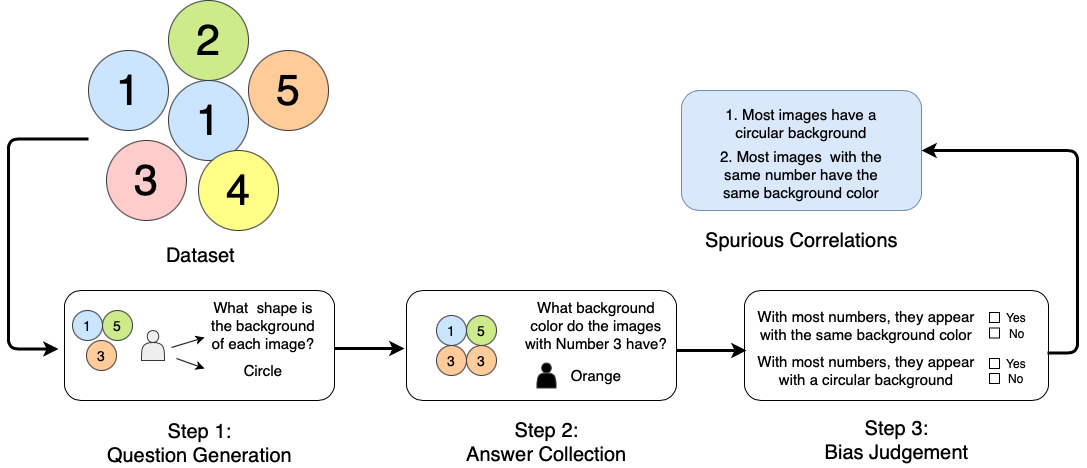
\includegraphics[scale=0.315]{crowdsourcing.png}
    \caption{Crowdsourcing approach to detect spurious correlations in image datasets, proposed by Hu et al. \cite{10.1145/3366423.3380063}}
    \label{fig:crowdsourcing}
\end{figure}

In summary, Crowdsourcing can be seen as an effective algorithm because it largely relies on human intuition to detect spurious correlations. An additional benefit of this approach is that it is conducted by working directly on the dataset which makes it superior to model explanations. \\
In both studies conducted by Hu et al. more than 10 volunteers per 100 images took part in the study. Even if one were to inspect only a small fraction of the dataset, one would need in excess of 100 volunteers! The fact that Crowdsourcing relies on such a large amount of volunteers is ambivalent. On the one hand, relying on multiple volunteers decreases the bias towards the perceptions of a small group and leads to finding more spurious correlations. However to most people needing to inspect a dataset such a large group of volunteers is unattainable and relying on humans to detect spurious correlations is time-consuming. Another problem with Crowdsourcing is that the output often contains incorrect detections. In the second study conducted by Hu et al. in which the volunteers inspected a car dataset two of the top 10 outputs were \enquote{No cars have rust} and \enquote{Each car is fueled by gasoline}. \\
In conclusion, Crowdsourcing is an effective approach to detect spurious correlations in image annotations but the high amount of time and effort it requires make it only applicable to frequently used datasets.


\subsection{Grad-CAM}
Grad-CAM highlights the parts of an image that contributed to a given classification by inspecting its final convolutional layer. An overview of Grad-CAM can be seen in \hyperref[fig:gradcam]{Figure 3}. \\
To generate an explanation for a given image with Grad-CAM, the image is first given to a CNN as its input and a class $c$ whose contribution should be explained needs to be specified. Grad-CAM then assigns a weight ${w_k}^c$ to each of the $n$ feature maps of the final convolutional layer of the given CNN with ${w_k}^c = \frac{1}{I \cdot J} \sum\limits_{i=1}^{I} \sum\limits_{j=1}^J \frac{\partial y^c}{\partial {A^k}_{i,j}}$.
This can be interpreted as the average importance of each entry of feature map $k$ to the classification of class $c$. The output of Grad-CAM is computed by adding up all $n$ feature maps multiplied by their respective weight and plugging them into a ReLU-function. Said differently, the output of Image $i$ with $c$ being the class of interest looks as follows: $O_{Grad-CAM, i, c} = ReLU(\sum\limits_{k=1}^N {w_k}^c \cdot A^k)$. ReLU is applied to filter out parts of the image that negatively contributed to the classification. Note that the output of Grad-CAM is of the same dimension as each feature map of the final convolutional layer which is usually much smaller than the dimension of the input image. \\
One advantage of Grad-CAM over other existing explanation algorithms is that its output is class-discriminative, i.e. that Grad-CAM only highlights those parts of the image that positively contributed to the specified class of interest. However since the output of Grad-CAM is of a smaller dimension than the input image its resolution is often not good enough to deliver a precise explanation. To combat this, Selvaraju et al. proposed a second approach named Guided Grad-CAM, which pointwise multiplies the output of a second explanation algorithm named Guided Backpropagation \cite{springenberg2015striving} where the output of Grad-CAM is first upscaled to the dimension of the input image. 
Guided Grad-CAM combines the benefits of Grad-CAM whose output is low resolution but class-discriminative and Guided Backpropagation which delivers an explanation in high resolution without being class-discriminative. This enables the visualization of fine-grained concepts which the CNN responds to like the stripes of the tiger-cat in \hyperref[fig:gradcam]{Figure 3}. \\
In conclusion, Grad-CAM is a visual explanation algorithm which can be used to detect spurious correlations in image datasets by inspecting the predictions of a CNN trained on the dataset of interest and checking whether the regions highlighted by Grad-CAM fit to concepts that spuriously correlate with the target class. For example a spurious correlation between gender and profession can be detected by checking whether Grad-CAM highlights the face of the depicted person or the clothing. 
A huge advantage of Grad-CAM is that it can be applied to any CNN which is currently the state-of-the-art model for most computer vision tasks. In addition, applying Grad-CAM requires no retraining which saves time in the process of detecting spurious correlations. Another benefit of Grad-CAM is the simplicity of its output: Since Grad-CAM explains the classification via a  simple heatmap, the explanation can be understood by anyone and no machine-learning expertise is needed. 
However, since Grad-Cam explains the classification of a model trained on the dataset of interest, it can only show the spurious correlations that the given model exploits. This can lead to problems because different models can rely on different (spurious) correlations when making their predictions.
Another problem of Grad-CAM is that one needs to inspect multiple explanations to confirm that the model relies on a certain concept when making its predictions. Since this needs to be done manually, it takes up most time in the detection process and slows it down considerably. Estimating the degree of a spurious correlation with Grad-CAM is also a challenge because Grad-CAM does not compute a value for a given spurious correlation. Research conducted by Tong \& Kagal \cite{tong2020investigating} has shown that most simple metrics fail to estimate the degree of a spurious correlation when using Grad-CAM because its output is noisy, i.e. it always highlights features which do not causally correlate with the target even if the dataset does not contain spurious correlations, only to a lesser extent.

\begin{figure}
    \centering
    \includegraphics[scale=0.057]{grad_cam_overview.png}
    \caption{Overview of Grad-CAM, proposed by Selvaraju et al. \cite{Selvaraju_2017_ICCV}. Grad-CAM explains a CNN-model by inspecting its final convolutional layer. The output of Grad-CAM can be pointwise multiplied with the output of an algorithm called Guided Backpropagation \cite{springenberg2015striving} to receive a more detailed explanation}
    \label{fig:gradcam}
\end{figure}


\subsection{TCAV}
TCAV \cite{pmlr-v80-kim18d} is an algorithm which detects spurious correlations by testing if a neural network trained on the dataset of interest relies on a user-defined concept when making its predictions. An overview of the algorithm can be seen in \hyperref[fig:tcav]{Figure 4} \\
\textbf{Step 1} requires the user to \textbf{define a concept} of interest $c$ (e.g. the stripes of a zebra or the face of a person). The user then collects a set of images that depict the concept and another set containing random images that do \textit{not} belong to the concept. Next, the user chooses a layer $l$ from the neural network which he wants to investigate. \\
In \textbf{Step 2} the images collected in Step 1 are fed into the neural network and a linear classifier is trained to separate the activations at layer $l$ that belong to the concept from the activations of the random images. The vector orthogonal to the decision boundary is the \textbf{concept activation vector} $v_c$ for the given concept $c$.  \\
In \textbf{Step 3} a \textbf{TCAV-Score} is assigned to the user-defined concept. To do so, a score $S_{c,k}(i)$ is assigned to each image containing class $k$ in the original dataset with $S_{c,k}(i) = \frac{\partial p_k(i)}{\partial v_c}$, meaning that $S_{c,k}(i)$ is the directional derivative of the prediction probability for class $k$ being present in image $i$ with regard to the concept activation vector. A positive $S_{c,k}(i)$ implies that the presence of concept $c$ in image $i$ positively contributed to is classification as class $k$.
The final TCAV-Score for a concept is $\frac{|i \in I_k: S_{c,k}(i) > 0 |}{|I_k|}$ where $I_k$ is the set of images in the dataset that contain class $k$. A concept with a high TCAV-Score is most likely a concept that the classifier relies on when making its predictions. \\
A huge benefit of TCAV is its flexibility towards model architecture: TCAV can be applied to any neural network and it is even possible to choose the layer which one wants to investigate. In addition, the algorithm can be automated so that all the user has to do is define the concept. This is important because it allows people without any machine-learning knowledge to investigate the model. However like Grad-CAM, TCAV is an algorithm that explains a given model an can therefore only detect spurious correlations which the given model exploits. An even bigger problem is that TCAV can only check if the model exploits a spurious correlation if the user has the assumption that this is the case. This means that spurious correlations which do not often occur and are therefore not assumed to be present in the dataset cannot be detected when detecting spurious correlations solely with TCAV. Another problem with TCAV is that it suffers from the \enquote{garbage in, garbage out}-principle: a poorly-defined concept can lead to a low TCAV-Score even if the concept is important. This can happen quite often because properly defining a concept can take time since one has to carefully select images that adequately represent the concept. Tong \& Kagal therefore propose to choose images that contain multiple concepts of interest to make the process of concept definition more efficient \cite{tong2020investigating}.

\begin{figure}
    \centering
    \includegraphics[scale=0.02]{grad_cam_overview.png}
    \caption{Overview of TCAV, proposed by Kim et al. \cite{pmlr-v80-kim18d}. TCAV can be used to determine if a user-defined concept significantly contributes to the predictions of a given neural network. The approach consists of three steps: first, the concept }
    \label{fig:tcav}
\end{figure}


\subsection{Comparing existing methods to detect spurious correlations}

\section{Mitigating the impact of spurious correlations}
\subsection{Why increasing model size exacerbates spurious correlations}
\subsection{How to mitigate the impact of spurious correlations between context and target}

\section{How to deal with datasets that might contain spurious correlations}

\section{Conclusion}

\printbibliography

\end{document}
